\section{General formulation of Murmuration}
\label{sec:general}

In his letter to Sutherland and Zubrilina, Sarnak proposed a general framework of murmuration \cite{sarnak} for \emph{families} of $L$-functions.
We explain his definition and its connection with the Katz--Sarnak philosophy \cite{katz1999zeroes,katz2023random}.
Also, we revisit previous murmuration results \cite{zubrilina2025murmurations,lee2025murmurations,sawin2025murmurations,wang2025murmurations} in this framework.
See also Lowry-Duda's survey note \cite{lowry2025murmurations}.

\subsection{Murmuration for families}

Let $\scF$ be a family of $L$-functions in a suitable sense (e.g. See \cite{sarnak2016families}).
For a smooth nonnegative function $\Phi : (0, \infty) \to \bR$ with compact support and $f : \scF \to \bC$, consider the $\Phi$-weighted average of $f$:
\begin{equation}
    \bE_{\pi \in \scF}[f; \Phi, N] := \frac{\sum_{\pi \in \scF} \Phi\left(\frac{N_\pi}{N}\right)f(\pi)}{\sum_{\pi \in \scF} \Phi\left(\frac{N_\pi}{N}\right)} = \frac{A_{\scF}(f; \Phi, N)}{A_{\scF}(1; \Phi, N)}
\end{equation}
where
\begin{equation}
    A_{\scF}(f; \Phi, N) := \sum_{\pi \in \scF} \Phi\left(\frac{N_\pi}{N}\right)f(\pi).
\end{equation}
Here $N_\pi$ is the ``conductor'' of $\pi$ (e.g. conductor of an elliptic curve or analytic conductor of an automorphic form).
When we order the family by the conductor, we say that $\scF$ has \emph{conductor dimension $\delta$} if
\begin{equation}
    \# \{\pi \in \scF : N_\pi \le N\} \sim \alpha N^\delta
\end{equation}
as $N \to \infty$ for some $\alpha > 0$ and $\delta = \delta(\scF) > 0$.
For such family, we have
\[
A_\scF(1; \Phi, N) \sim \alpha \delta N^\delta \int_0^\infty \Phi(x) x^\delta \frac{\dd x}{x}.
\]

Most of the known murmuration results consider the function
\begin{equation}
    f(\pi) = a_\pi(p) := \sqrt{p} \lambda_\pi(p)
\end{equation}
for a given prime $p$, where $\lambda_\pi(p)$ is the normalized trace of Frobenius at $p$ so that the Ramanujan--Petersson conjecture says $|\lambda_\pi(p)| \le n$ for $\GL_n$ automorphic forms $\pi$.
Furthermore, if $\scF$ is self-dual, then $a_\pi(p)$ is real and the global root number $w_\pi$ is either $1$ or $-1$.
Then we can separate by root number and consider the averages
\begin{equation}
    \bE_{\pi \in \scF^w} [a_\pi(p); \Phi, N]
\end{equation}
for $w \in \{\pm 1\}$ and $\scF^w = \{\pi \in \scF : w_\pi = w\}$.


\begin{definition}
A continuous function $M_\Phi : (0, \infty) \to \bR$ is a \emph{murmuration function for $\scF$ with weight $\Phi$} if there is $0 \le \gamma < 1$ such that for $P \sim N$
\begin{equation}
    \label{eqn:sarnak_murmuration}
    \bE_{\pi \in \scF} [a_\pi(p);\Phi, N] = M_\Phi\left(\frac{p}{N}\right) + R(p, N)
\end{equation}
where the local oscillating term $R(p, N)$ satisfies\footnote{In \cite{sarnak}, he considered local average over primes $P-H \le p \le P + H$ instead of $P \le p \le P + H$, but most of the latter works seems to follow one-sided averaging.}
\begin{equation}
    \label{eqn:sarnak_local_avg}
    \bE_{P \le p \le P + H} [R(p, N)] = \frac{\sum_{P \le p \le P + H} R(p, N)}{\sum_{P \le p \le P + H} 1} = o(1)
\end{equation}
for $H = o(N)$.
\end{definition}
Equation \eqref{eqn:sarnak_local_avg} is the local averaging over $p$ of length at least $N^\gamma$ and less than $N$.
The smaller $\gamma$ we can take, the more visible $M_\Phi$ is.
In particular, $\gamma = 0$ means that no local averaging is needed.
He conjectured that if
\begin{equation}
    \label{eqn:sarnak_local_thres}
    \delta + \gamma > 1
\end{equation}
then the local oscillating term $R(p, N)$ will vanish as $N \to \infty$.
In particular, we may not need local averaging if $\delta > 1$.

The function $M_\Phi$ is supposed to have a form of
\begin{equation}
    \label{eqn:sarnak_zubrilina_density}
    M_\Phi(y) = \frac{\int_0^{\infty} \Phi(u) M\left(\frac{y}{u}\right) u^\delta \frac{\dd u}{u}}{\int_0^{\infty} \Phi(u) u^\delta \frac{\dd u}{u}}.
\end{equation}
for some universal $M : (0, \infty) \to \bR$.
If such a function (more generally, distribution) exists, we call it as \emph{Zubrilina murmuration density for $\scF$}, denoted as $Z_{\scF}$.
It might be a distribution on $C_c^\infty((0, \infty))$ rather than a function.



\subsection{Katz--Sarnak philosophy}


Katz and Sarnak \cite{katz1999zeroes,katz2023random} studied statistics of zeros of $L$-functions via random matrix models.
In particular, they considered \emph{one-level density} of low-lying zeros: for an even function $\phi$ with rapid decay as $|x| \to \infty$, the one-level density of a family $\scF$ is
\begin{equation}
    \OLD(\scF; \phi) = \lim_{N \to \infty} \bE_{\pi \in \scF(N)} \left[\sum_{\gamma_\pi} \phi\left(\frac{\gamma_\pi \log N}{2 \pi}\right)\right]
\end{equation}
where $\scF(N) := \{\pi \in \scF: N_\pi = N\}$ and $\gamma_\pi$ runs through the ordinates of nontrivial zeros of $L(s, \pi)$ on the critical line, i.e. $L\left(\frac{1}{2} + i\gamma_\pi, \pi\right) = 0$.
The factor $\frac{\log N}{2\pi}$ guarantees that the nontrivial zeros have unit spacing on average.
Katz--Sarnak philosophy claims that there is a measure $W_\scF$ coming from matrices related to the ``type'' of $\scF$ such that
\begin{equation}
    \OLD(\scF; \phi) = \int_{\bR} \what{\phi}(x) \what{W_\scF}(x) \dd x
\end{equation}
for any nice test function $\phi$.
We say that $\scF$ has orthogonal/symplectic/unitary symmetry type if $W_\scF$ comes from one of the orthogonal/symplectic/unitary groups.
More precisely, let $G(N)$ be one of the ``ensembles'' in \cite[Table 1]{katz1999zeroes}, e.g. $G(N) = \mathrm{U}(N)$, the compact group of $N \times N$ unitary matrices.
Let $\dd A$ be a Haar measure on $G(N)$, and let $e^{i \theta_1(A)}, \ldots, e^{i \theta_{N}(A)}$ be the eigenvalues of $A \in G(N)$, where $0 \le \theta_1(A) \le \cdots \le \theta_N(A) < 2\pi$.
Let
\[
\Delta(A)[a, b]  := \#\{\theta(A) : e^{i\theta(A)}\text{ is an eigenvalue of }A \text{ and } \frac{\theta(A)N}{2\pi} \in [a, b]\}.
\]
Then we have a density function $W_G : \bR \to \bR_{\ge 0}$ such that for any interval $[a, b] \subset \bR$,
\[
\lim_{N \to \infty} \int_{G(N)} \Delta(A)[a, b] \dd A = \int_a^b W_G(x) \dd x.
\]
For example, $W_G$ for unitary/orthogonal/symplectic groups are given by
\begin{align}
    \label{eqn:WG}
    W_{\mathrm{U}}(x) &= 1, \\
    W_{\mathrm{SO(+)}(x)} &= 1 + \frac{\sin(2\pi x)}{2\pi x}, \\
    W_{\mathrm{SO(-)}(x)} &= 1 - \frac{\sin(2\pi x)}{2\pi x} + \delta_0(x), \\
    W_{\mathrm{Sp}}(x) &= 1 - \frac{\sin(2\pi x)}{2\pi x}.
\end{align}

One such example is the following theorem on the family of Hecke eigenforms by Iwaniec, Luo, and Sarnak \cite{iwaniec2000low}, showing that the family has orthogonal symmetry type.
\begin{theorem}[Iwaniec--Luo--Sarnak \cite{iwaniec2000low}]
    Assume GRH. Let $\phi$ be an even Schwartz function with $\supp(\what{\phi}) \subset (-2, 2)$.
    Let $H_k^\pm$ be a set of Hecke eigenforms of weight $k$ and root number $\epsilon = \pm 1$.
    Then
    \begin{equation}
        \OLD(H_k^\pm; \phi) = \int_{\bR} \what{\phi}(x) \what{W_{\SO(\pm)}}(x) \dd x
    \end{equation}
\end{theorem}
There is an explicit formula relating the summation over zeros of $L$-functions and over primes, which is given by \cite[Section 4]{iwaniec2000low}
\begin{align*}
    \sum_{\gamma_\pi} \phi\left(\frac{\gamma_\pi \log N}{2\pi}\right) &= C - 2 \sum_p \sum_{\nu \ge 1} \left(\sum_{j} \alpha_j(p)^\nu\right) \what{\phi}\left(\frac{\nu \log p}{\log N}\right) \frac{\log p}{p^{\nu/2} \log N}
\end{align*}
and since $\what{\phi}$ is compactly supported, the main contribution comes from $\nu = 1$ summand, so we are mostly interested in 
\begin{equation}
    \sum_{p} \frac{\lambda_\pi(p)}{p^{1/2}} \what{\phi}\left(\frac{\log p}{\log N}\right) \frac{\log p}{\log N} 
\end{equation}
The Fourier transforms of \eqref{eqn:WG} are
\begin{equation}
    \what{W_{\SO(+)}}(y) = \delta_0(y) + \frac{2 - \1_{[-1, 1]}(y)}{2}, \quad \what{W_{\SO(-)}}(y) = \delta_0(y) + \frac{\1_{[-1, 1]}(y)}{2}
\end{equation}
and there are obvious discontinuities at $y = \pm 1$.
Hence, at least roughly, this suggests that the behavior of the average of $\lambda_\pi(p) / p^{1/2}$ with $p \sim N^a$ changes at $a = 1$.
Katz--Sarnak philosophy suggests that, when $\scF$ is of symplectic type, then
\[
\bE_{p \sim N^a} \left[ \bE_{\pi \in \scF} [a_\pi(p); \Phi, N]\right] \to \begin{cases}
    0 & a < 1 \\ -\frac{1}{2} & a > 1
\end{cases}
\]
and when $\scF$ is of orthogonal type,
\[
\bE_{p \sim N^a} \left[ \bE_{\pi \in \scF^w} [a_\pi(p); \Phi, N]\right] \to \begin{cases}
    0 & a < 1 \\ \frac{w}{2} & a > 1
\end{cases}
\]
(see \cite[eq. (7')]{sarnak}).
Each $a < 1$ and $a > 1$ corresponds to the limit of $M_\Phi(y)$ as $y \to 0$ and $y \to \infty$.




\subsection{Revisiting the murmuration theorems}

Let's see how the existing works on murmurations fit into the above framework.

\subsubsection{Dirichlet characters}

In case of Dirichlet characters \cite{lee2025murmurations}, the family of even/odd \emph{complex} Dirichlet characters are not self-dual, so it does not fit into Sarnak's framework precisely.
Still, we can observe and prove murmuration phenomena for such a family, where the density function is much simpler compared to other families.
Also, for each prime $P$, there are $\phi(P) = P-1$ primitive characters modulo $P$, so there are about $\frac{CN^2}{\log N}$ primitive Dirichlet characters of prime conductors $\le N$ for some constant $C > 0$, which means that the conductor dimension of the family is $2-\epsilon$\footnote{The $\log N$ factor disappears if we consider all conductors that are not necessarily prime, and the conductor dimension becomes $2$. See \cite[Section 6]{lee2025murmurations} for the version including composite conductors.}.
In particular, \eqref{eqn:sarnak_local_thres} suggests that we don't need any further local averaging for the family, which is indeed the case of Theorem \ref{thm:lop_dirichlet}.
Note that normalization used in Theorem \ref{thm:lop_dirichlet} is also different from the one Sarnak suggested.

For the quadratic characters, local averaging is included in Theorem \ref{thm:lop_dirichlet_quad} over $X^{\gamma}$-many primes with $\frac{3}{4} < \gamma < 1$.
Since the number of square-free odd numbers up to $X$ is $\Theta(X)$, the conductor dimension of the family $\scF = \{\chi_{8d} : d\text{ odd and square-free}\}$ is $\delta = 1$ so we may only need local averaging over $X^{\epsilon}$-many primes for any $\epsilon > 0$ from \eqref{eqn:sarnak_local_thres}.
From Theorem \ref{thm:lop_dirichlet_quad}, the Zubrilina density for the family is
\begin{equation}
    Z_{\scF}(y) = \frac{\sqrt{2}}{2} \sum_{\substack{a \ge 1 \\ \gcd(a, 2) = 1}} \frac{\mu(a)}{a^2} \sum_{m \ge 1} (-1)^m \cos\left(\frac{\pi m^2}{a^2 y} - \frac{\pi}{4}\right).
\end{equation}
Note that this is not an actual function but rather a distribution, since the inner sum in $m$ diverges for the most of $y$'s.
It seems that the distribution is a certain combination of delta functions at rational points, although it is not mentioned in \cite{lee2025murmurations}.
Figure \ref{fig:dirichlet_density} shows that it might be supported at $0, \frac{1}{5}, \frac{3}{5}, \frac{4}{5}, 1$, etc.

\begin{figure}
    \centering
    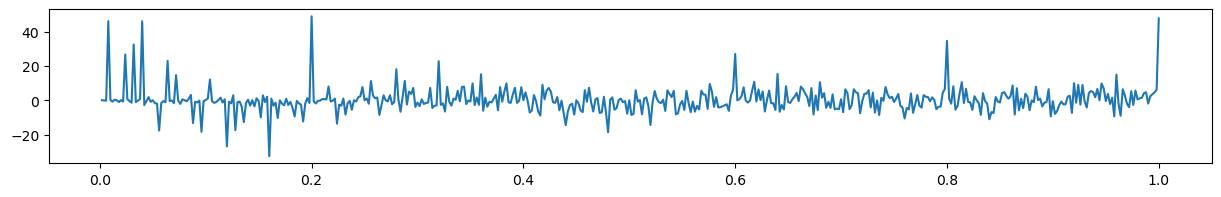
\includegraphics[width=0.7\textwidth]{src/dirichlet_density.png}%
    \caption{Plot of $Z_{\scF}(y)$ for $y = \frac{i}{500}$ with $1 \le i \le 500$, truncated at $a < 200$ and $m \le 100$.}
    \label{fig:dirichlet_density}
\end{figure}

\subsubsection{Modular forms}

It is known that the dimension of the space of newforms of fixed weight $k$ and level $\Gamma_0(N)$ is asymptotically $\frac{45(k-1)N}{\pi^2}$ \cite[Theorem 8]{martin2005dimensions}.
It implies that the number of newforms of fixed weight $k$ and level $\Gamma_0(M)$ for square-free $M \le N$ is asymptotically $c_k N^2$ for a constant $c_k > 0$, so the conductor dimension of the family is $2 > 1$.
From Sarnak's suggestion \eqref{eqn:sarnak_local_thres}, we expect that we don't need any further local averaging, and this is indeed the case of Theorem \ref{thm:zubrilina_modform} and \ref{thm:zubrilina_geom}.

Also, she studied several properties of her density function $\cM_k$.
In particular, for a compactly supported smooth function $\Phi$ on $(0, \infty)$, she proved that the function
\begin{equation}
    \cM_{\Phi}^k(y) := \frac{\int_0^\infty \cM_k\left(\frac{y}{u}\right) \Phi(u) u^2 \frac{\dd u}{u}}{\int_0^\infty \Phi(u) u^2 \frac{\dd u}{u}}
\end{equation}
is continuous in $y$ and
\[
\lim_{y \to 0^+} \cM_k(y) = 0, \quad \lim_{y \to \infty}\cM_k(y) = \frac{1}{2}.
\]
This is compatible with Katz--Sarnak philosophy, since the family of modular forms has orthogonal symmetry type.

\subsubsection{Elliptic curves}

The conductor dimension of a family of elliptic curves ordered by \emph{conductor} is conjecturally $\frac{5}{6}$ \cite{shankar2019families}, so we may need local averaging over $X^{1/6 + \epsilon}$-many primes from \eqref{eqn:sarnak_local_thres}, although it is clear that there's an obvious murmuration pattern in the case (that's the first ever murmuration oberved in number theory!).
In fact, it seems that the noise may still exist even if we increase the conductor range, as partially shown in Figure \ref{fig:sutherland_elliptic_dyadic} (Sutherland computed murmuration up to the range of $[250000, 500000]$ \cite{sutherlandletter}, which is not reproduced in Figure \ref{fig:sutherland_elliptic_dyadic} due to the computational limitation).
Figure \ref{fig:elliptic_dyadic_local_avg} shows the murmuration of non-CM elliptic curves with conductor in $[2^k, 2^{k+1})$ and primes $p < 2^k$ for $k = 12, \dots, 16$ weighted by root numbers, without (resp. with) local averaging of $X^\gamma = X^{\frac{1}{2}}$-many primes.
Smaller $\gamma$ gives less visible (purple) curves with larger noise.

\begin{figure} 
    \begin{subfigure}{1.0\textwidth}
        \centering
        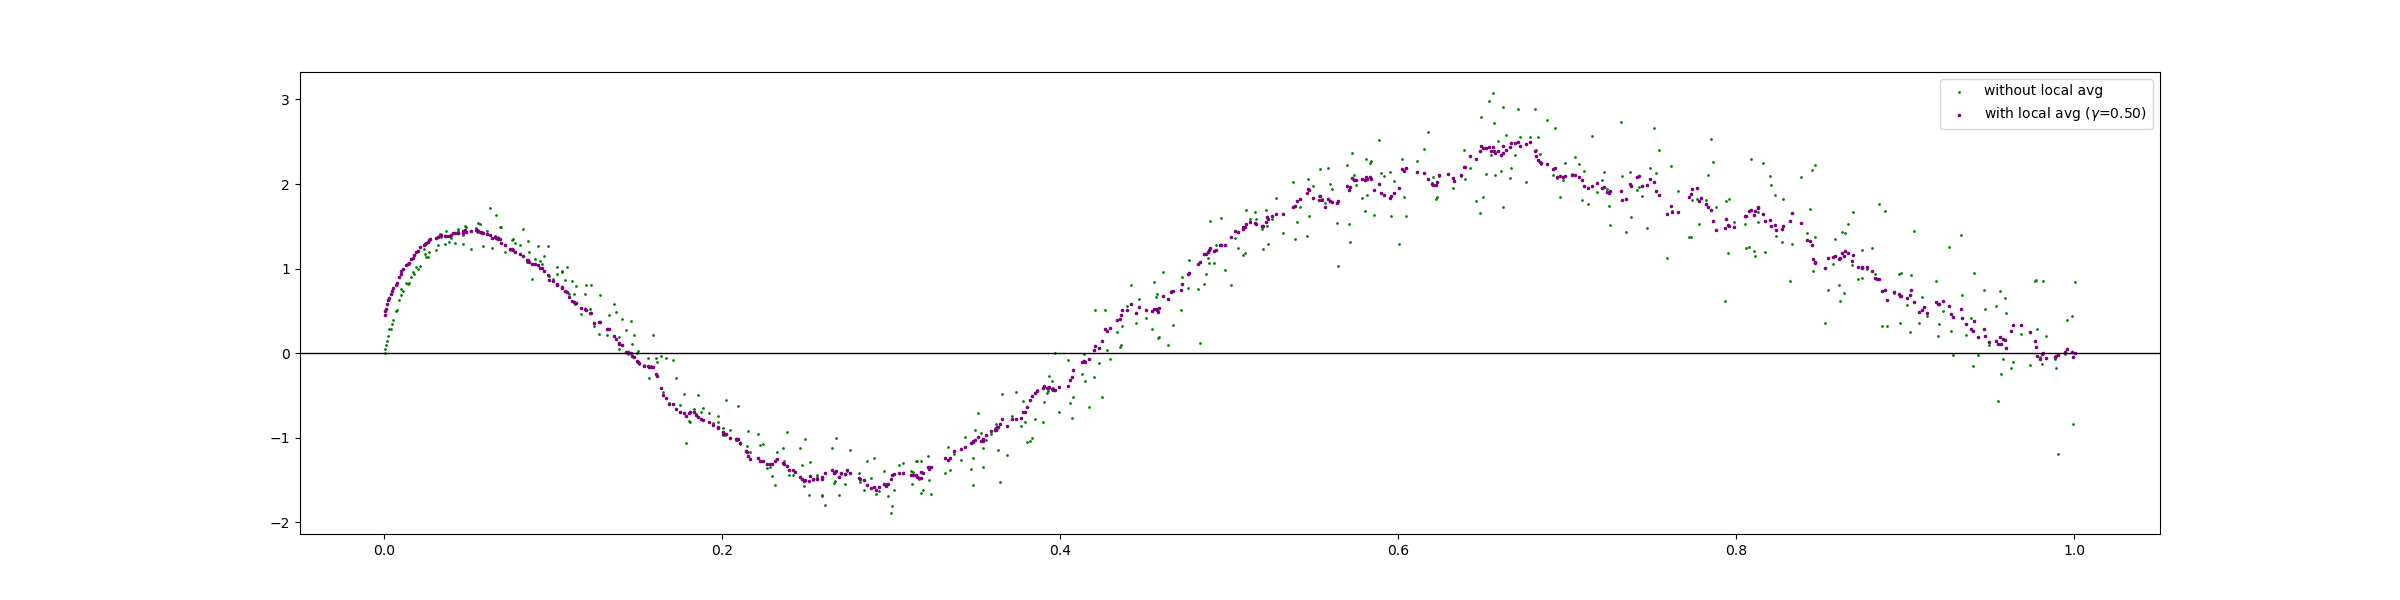
\includegraphics[width=\textwidth]{src/ec_local_4096.png}%
        \label{fig:ec_local_4096}
    \end{subfigure}
    
    \begin{subfigure}{1.0\textwidth}
        \centering
        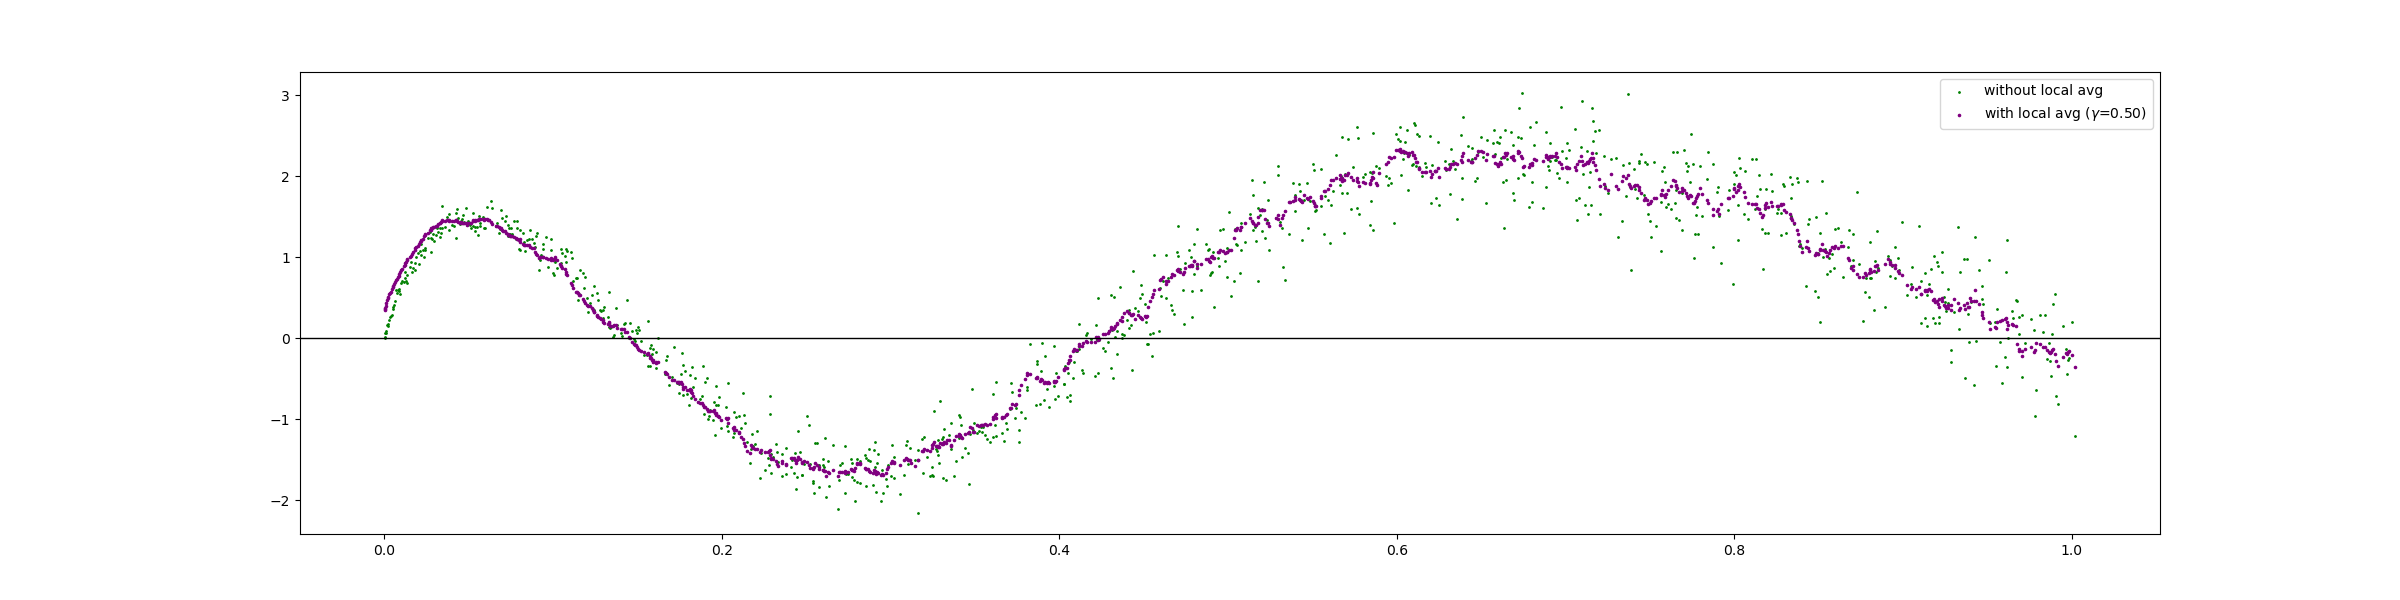
\includegraphics[width=\textwidth]{src/ec_local_8192.png}%
        \label{fig:ec_local_8192}
    \end{subfigure}

    \begin{subfigure}{1.0\textwidth}
        \centering
        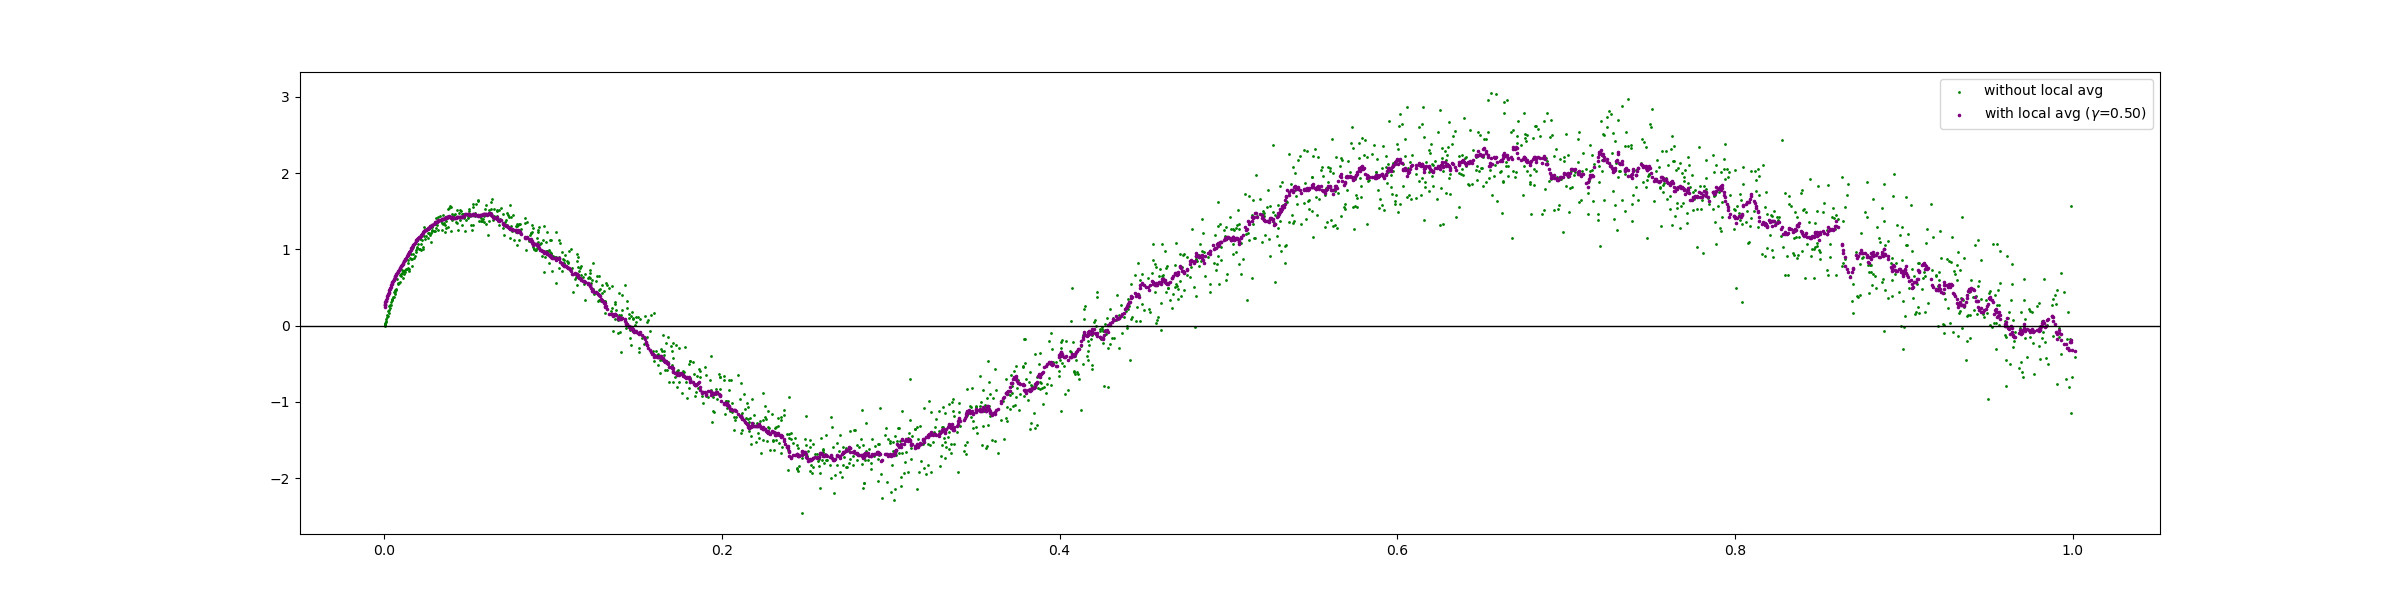
\includegraphics[width=\textwidth]{src/ec_local_16384.png}%
        \label{fig:ec_local_16384}
    \end{subfigure}

    \begin{subfigure}{1.0\textwidth}
        \centering
        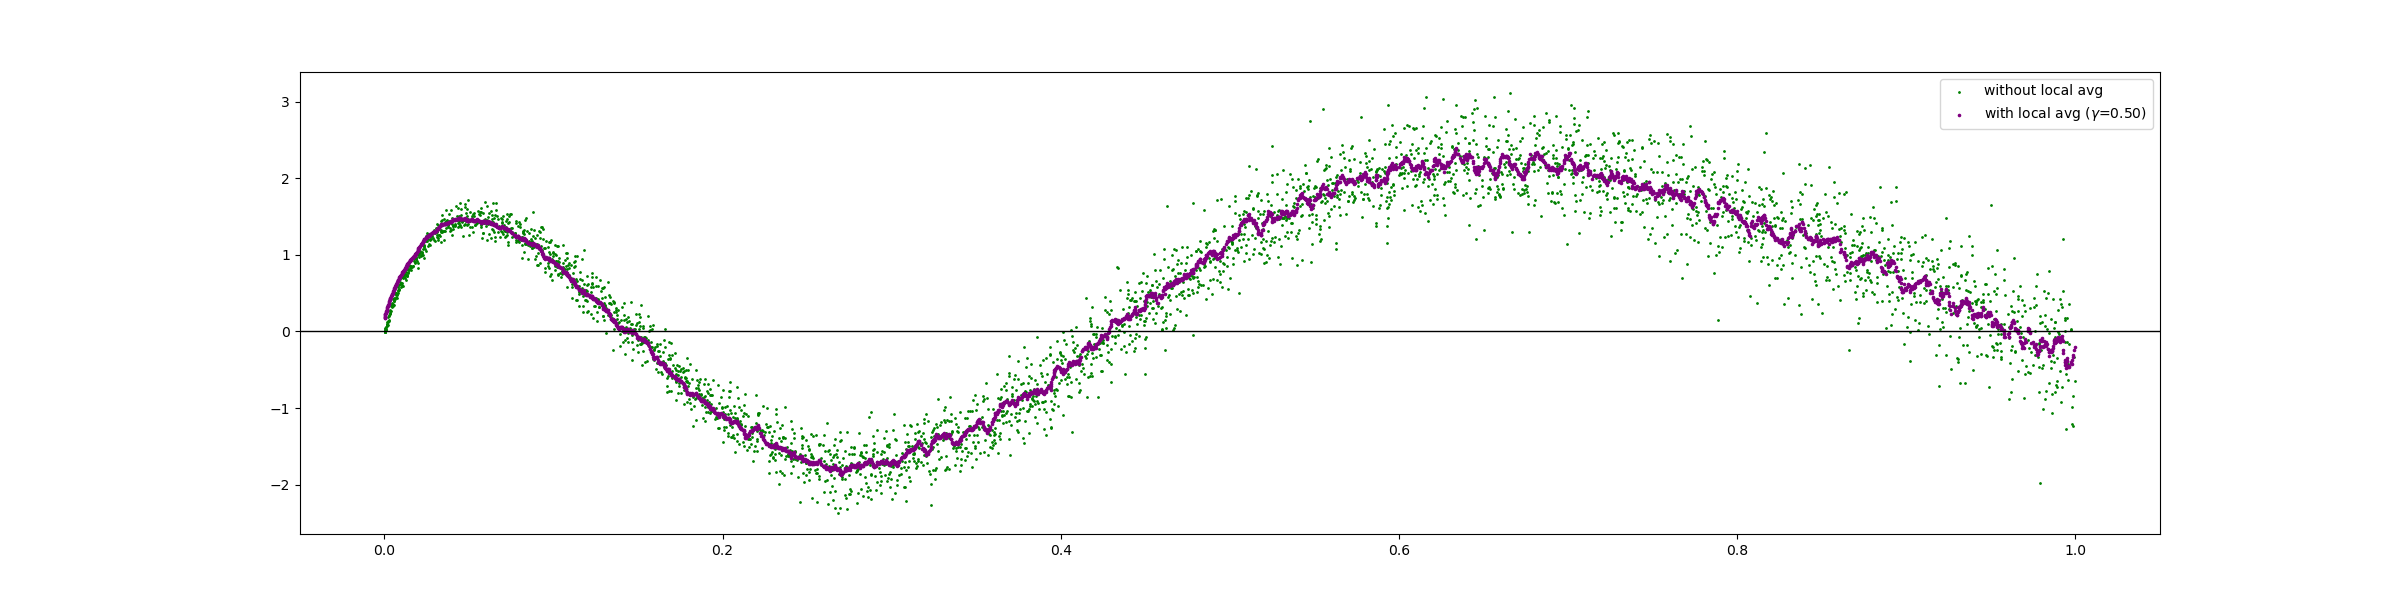
\includegraphics[width=\textwidth]{src/ec_local_32768.png}%
        \label{fig:ec_local_32768}
    \end{subfigure}

    \begin{subfigure}{1.0\textwidth}
        \centering
        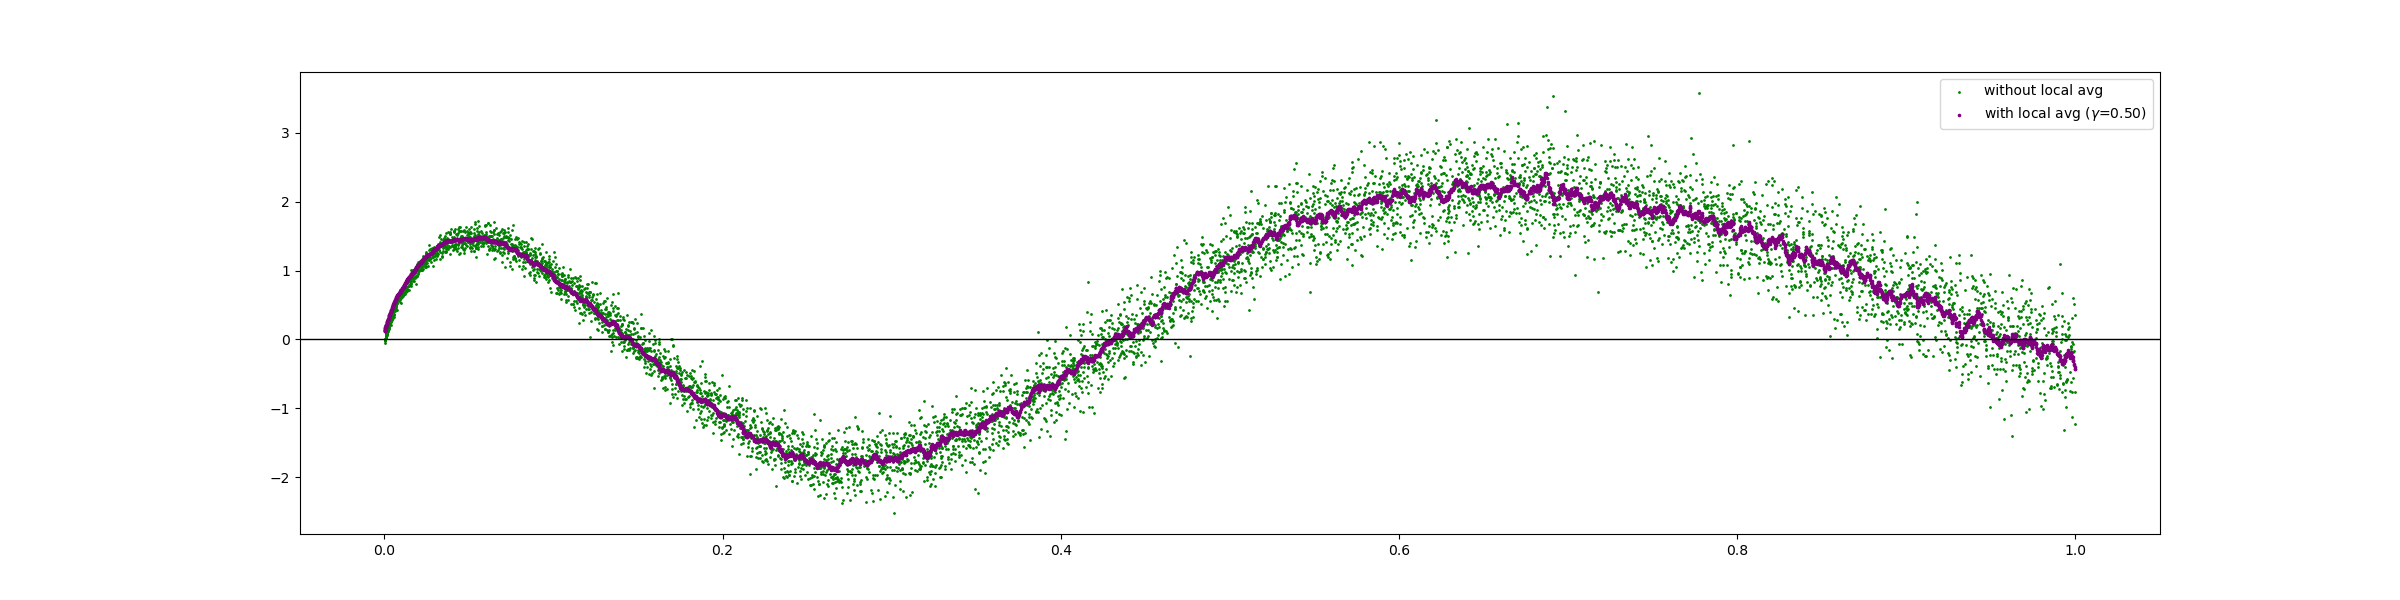
\includegraphics[width=\textwidth]{src/ec_local_65536.png}%
        \label{fig:ec_local_65536}
    \end{subfigure}
    \caption{Murmuration of non-CM elliptic curves with conductor in $[2^{k}, 2^{k+1})$ and primes $p < 2^{k}$ for $k = 12, \dots, 16$ weighted by root numbers, without (resp. with) local averaging of $X^\gamma = X^{\frac{1}{2}}$-many primes.}
\label{fig:elliptic_dyadic_local_avg}
\end{figure}


In the case of \cite{sawin2025murmurations}, the conductor dimension of a family of elliptic curves ordered by heights is also (non-conjecturally) $\frac{5}{6}$, so we may need further local averaging over $X^{1/6 + \epsilon}$ many primes.
The local averaging introduced in Theorem \ref{thm:sawin-sutherland} is slightly different from Sarnak's suggestion, since they take a local average over $\Theta(N_E)$-many primes, not $O(H_E^{1/6 + \epsilon})$.


\subsection{Hecke characters of imaginary quadratic fields}


For each $D \equiv 3 \Mod{4}$, the number of Hecke characters of $\mathrm{Cl}(\bQ(\sqrt{-D}))$ is $h(-D)$, and the class number formula
\[
h(-D) = \frac{\sqrt{D}}{\pi} L(1, \chi_{-D})
\]
with the estimates $|D|^{-\epsilon} \ll L(1, \chi_{-D}) \ll |D|^{\epsilon}$\footnote{The lower bound is Siegel's theorem, while the upper bound follows from the Pólya--Vinogradov inequality.} implies that the conductor dimension of $\scF$ is $\frac{3}{2}$.
In particular, it is larger than $1$, so we may not need any local averaging from \eqref{eqn:sarnak_local_thres}.
However, we still include it in Theorem \ref{thm:wanglocal} to remove the dependence on $p$ in the main term of Theorem \ref{thm:wang}.
The main term
\[
M(y) = \overline{c} \sum_{1 \le m < 2 \sqrt{y}} \overline{M}_m(y) + M_-(y)
\]
in Theorem \ref{thm:wanglocal} is the murmuration density for the family $\scF$, so we expect that
\begin{equation}
    \bE_{P \le p \le P + N}\left[\bE_{\psi \in \scF} [\sqrt{p} a_\psi(p); \Phi, N]\right] = M_\Phi\left(\frac{p}{N}\right) + o(1)
\end{equation}
for a compactly supported smooth function $\Phi$ on $(0, \infty)$ and
\begin{equation}
    M_\Phi(y) = \frac{\int_0^\infty M\left(\frac{y}{u}\right) \Phi(u) u^{3/2} \frac{\dd u}{u}}{\int_0^\infty \Phi(u) u^{3/2} \frac{\dd u}{u}}.
\end{equation}
The family is expected to have a symplectic symmetry type \cite{fouvry2003low,sarnak2016families}, so we expect
\[
\lim_{y \to 0^+} M_\Phi(y) = 0, \quad \lim_{y \to \infty} M_\Phi(y) = -\frac{1}{2}
\]
and this is Theorem 3 of \cite{wang2025murmurations}.
(Recall that Zubrilina's family has an orthogonal symmetry type.)